\documentclass[a4paper, 12pt]{article}%тип документа

%отступы
\usepackage[left=2cm,right=2cm,top=2cm,bottom=3cm,bindingoffset=0cm]{geometry}
\setlength{\parindent}{5ex}

%Русский язык
\usepackage[T2A]{fontenc} %кодировка
\usepackage[utf8]{inputenc} %кодировка исходного кода
\usepackage[english,russian]{babel} %локализация и переносы

%Вставка картинок
\usepackage{graphicx}
\graphicspath{{pictures/}}
\DeclareGraphicsExtensions{.pdf,.png,.jpg}

%Графики
\usepackage{pgfplots}
\pgfplotsset{compat=1.9}

%Математика
\usepackage{amsmath, amsfonts, amssymb, amsthm, mathtools}

%Таблицы
\usepackage{longtable} 
\usepackage{float}

%Римские цифры
\newcommand{\RomanNumeralCaps}[1]{\uppercase\expandafter{\romannumeral#1}}

\usepackage{multirow}


\begin{document}
	\begin{titlepage}
		\begin{center}
			\textsc{Федеральное государственное автономное образовательное учреждение высшего образования«Московский физико-технический институт (национальный исследовательский университет)»\\[5mm]
			}
			
			\vfill
			
			\textbf{Отчёт по лабораторной работы 3.4.5\\[3mm]
				Петля гистерезиса (динамический метод)
				\\[50mm]
			}
			
		\end{center}
		
		\hfill
		\begin{minipage}{.5\textwidth}
			Выполнил студент:\\[2mm]
			Сериков Василий Романович\\[2mm]
			группа: Б03-102\\[5mm]
			
		\end{minipage}
		\vfill
		\begin{center}
			Москва, 2022 г.
		\end{center}
		
	\end{titlepage}
	
	\newpage
	\textbf{Аннотация}\\
	
	
	\textbf{Цель работы: }\\
	
	Изучение петель гистерезиса различных ферромагнитных материалов в переменных полях.\\
	
	\textbf{В работе используются: }\\
	
	Автотрансформатор, понижающий трансформатор, интегрирующая цепочка амперметр, электронный осциллограф, делитель напряжения, тороидальные образцы с двумя обмотками.\\
	
	\textbf{Теоретические сведения: } \\
	
	Если состояние некоторой системы зависит не только от мгновенных
	значений внешних параметров, но от истории их изменений, говорят, что
	в системе имеет место гистерезис.
	
	В данной работе кривые гистерезиса ферромагнитных материалов изучаются в поле частоты $\nu_0$ = 50 Гц с помощью электронного осциллографа.
	
	Магнитная индукция B и напряжённость поля H в ферромагнитном материале неоднозначно связаны между собой: индукция зависит
	не только от напряжённости, но и от предыстории образца. Связь между B и H типичного ферромагнетика иллюстрирует рис.1.
	
	Если к ферромагнитному образцу прикладывать переменное внешнее
	магнитное поле, то его состояние на плоскости H-B будет изменяться
	по замкнутой кривой — петле гистерезиса. Размер петли определяется
	максимальным значением напряжённости H в цикле (напр., петля AA',
	обозначенная пунктиром на рис. 1). Если амплитуда напряжённости достаточно велика, то образец будет периодически достигать насыщения,
	что на рисунке соответствует кривой CEFC'E'F'C (предельная петля
	гистерезиса). Пересечение предельной петли с вертикальной осью соответствует остаточной индукции $B_r$, пересечение с горизонтальной осью — коэрцитивному полю $H_c$. Крайние точки петель, соответствующие амплитудным значениям H (например, точка A на рис. 1), лежат на начальной кривой намагничивания (OAC).
	
	
	\begin{figure}[h]
		\center{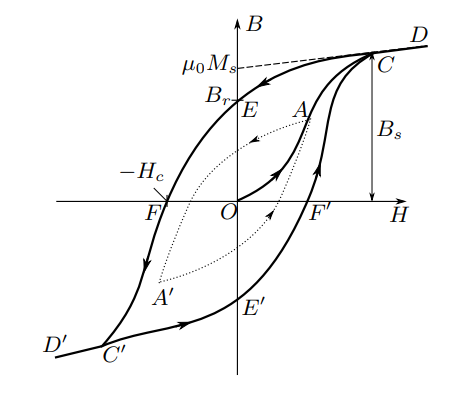
\includegraphics [scale=0.8]{photo1.png}}
		\caption{Петля гистерезиса ферромагнетика.}
	\end{figure}
	
	\newpage
	
	Магнитную индукцию B удобно
	определять с помощью ЭДС, возникающей при изменении магнитного
	потока $\Phi$ в катушке, намотанной на образец. Пусть катушка c N витками плотно охватывает образец сечением S, и индукция B в образце
	однородна, тогда выражение для В будет таким:
	
	\begin{equation}
	|B|=\dfrac{1}{SN_{и}}\int{\mathcal{E}}dt
	\end{equation}
	
	Для интегрирования сигнала применяют интегрирующие схемы (рис. 2)
	
	\begin{figure}[h]
		\center{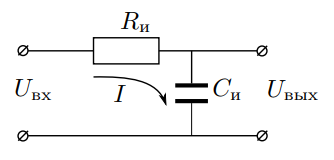
\includegraphics [scale=1]{photo2.png}}
		\caption{Схема RC-цепи.}
	\end{figure}
	
	Входное и выходное сопротивление связаны соотношением
	
	\begin{equation}
		U_{\text{вых}}\simeq\dfrac{1}{\tau}\int U_{\text{вх}}dt
	\end{equation}
	
	\begin{equation}
		U_{\text{вых}}=\dfrac{U_{\text{вх}}}{\tau\Omega}
	\end{equation}
	
	Тогда для В получим:
	
	\begin{equation}
		|B|=\dfrac{1}{SN_{\text{и}}}\int U_{\text{вх}}dt=\dfrac{\tau_{\text{и}}}{SN_{\text{и}}}U_{\text{вых}}
	\end{equation}
	
	где $\tau_{\text{и}} = R_{\text{и}} C_{\text{и}} -$ постоянная времени RC-цепочки.\\
	
	
	\textbf{Экспериментальная установка: }\\
	
	Схема установки изображена на рис. 3. Напряжение сети - 220 В, частота - 
	50 Гц. С помощью трансформаторного блока Т, состоящего из регулировочного автотрансформатора и разделительного понижающего трансформатора это напряжение подаётся на намагничивающую обмотку $N_0$ исследуемого
	образца.
	
	В цепь намагничивающей катушки, на которую подаётся некоторое
	напряжение $U_0$, последовательно включено сопротивление $R_0$. Напряжение на $R_0$, равное $U_R$. = $R_0 I_0$., где $I_0$. — ток в намагничивающей обмотке $N_0$., подаётся на канал X осциллографа. Связь напряжённости H в образце и тока $I_0$. рассчитывается по теореме о циркуляции.
	
	Для измерения магнитной индукции B с измерительной обмотки $N_{\text{и}}$.
	на вход RC-цепочки подаётся напряжение $U_{\text{и}}$ ($U_{\text{вх}}$), пропорциональное
	производной $dB/dt$ С интегрирующей ёмкости $C_{\text{и}}$ снимается напряжение $U_{c}$ ($U_{\text{вых}}$), пропорциональное величине B, и подаётся на вход Y
	осциллографа. Значение индукции поля B рассчитывается по формуле (3).
	
	\newpage
	
	\begin{figure}[h]
		\center{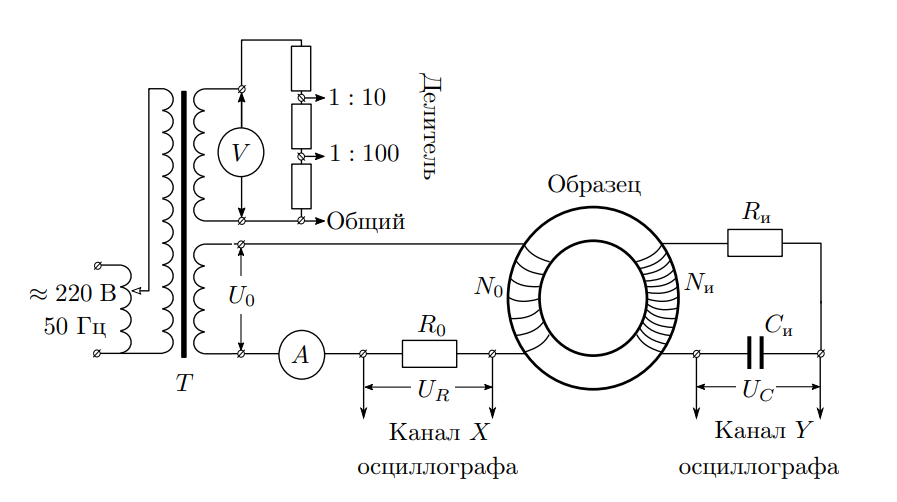
\includegraphics [scale=1]{photo3.png}}
		\caption{Схема экспериментальной установки.}
	\end{figure}
	
	
	\textbf{Результаты измерений и обработка данных:}
	
	\begin{enumerate}
		
	\item Запишем начальные данные и погрешности.
	
	$R_{\text{и}} = 20$ кОм,				
	$C_{\text{и}} = 20$ мкФ,				
	$ R_0 = 0,2$ Ом
	$\sigma_x = \frac{K_x}{5}$
	$\sigma_y = \frac{K_y}{5}$
	
			\begin{longtable} {|c|c|c|c|c|}
			\hline
			  & $N_0$ &  $ N_u $ & $ S $, см$^2$ & $2\pi R$, см      \\ \hline
			Феррит & 45 & 400 & 3 & 25\\ \hline
			Кремнистое железо & 20  & 200 &  2  & 11   \\ \hline
			Пермаллой & 15 & 300&  0,66   &  14,1 \\ \hline
			\caption{Начальные данные}
		\end{longtable}
		
		
	\item Получим кривую гистерезиса и снимем параметры ЭО для каждого образца
	
	\textbf{Пермаллой: }\\
	$K_x = 20$ мВ/дел\\
	$K_y = 50$ мВ/дел\\
	$2X_s = (10\pm0,2)K_x$ - полная ширина предельной петли\\
	$2Y_s = (3,4\pm0,2)K_y$	- полная высота предельной петли\\
	$2X_c = (5\pm0,2)K_x$ - двойная амплитуда для коэрцитивного поля\\
	$2Y_r = (3,4\pm0,2)K_y$	- двойная амплитуда остаточной индукции\\
	
	\textbf{Феррит: }\\
	$K_x = 20$ мВ/дел\\
	$K_y = 20$ мВ/дел\\
	$2X_s = (7,2\pm0,2)K_x$ - полная ширина предельной петли\\
	$2Y_s = (5\pm0,2)K_y$	- полная высота предельной петли\\
	$2X_c = (0,8\pm0,2)K_x$ - двойная амплитуда для коэрцитивного поля\\
	$2Y_r = (2,4\pm0,2)K_y$	- двойная амплитуда остаточной индукции\\
	\textbf{Кремнистое железо: }\\
	$K_x = 0,1$ В/дел\\
	$K_y = 20$ мВ/дел\\
	$2X_s = (7,6\pm0,2)K_x$ - полная ширина предельной петли\\
	$2Y_s = (7,4\pm0,2)K_y$	- полная высота предельной петли\\
	$2X_c = (1,2\pm0,2)K_x$ - двойная амплитуда для коэрцитивного поля\\
	$2Y_r = (3,2\pm0,2)K_y$	- двойная амплитуда остаточной индукции\\
	
	\item Проведем измерения начальной кривой намагничивания для каждого образца.
	
	\begin{longtable} {|c|c|c|c|c|c|c|c|c|}
		\hline
		№ & 1 & 2 & 3 & 4 & 5 & 6 & 7 & 8 \\ \hline 
		$x, $ дел & 4,0 & 3,6 & 3,0 & 2,2 & 1,8 & 1,7 & 1,6 & 1,2 \\ \hline
		$y, $ дел & 1,8 & 1,7 & 1,6 & 1,4 & 1,2 & 0,8 & 0,4 & 0,1 \\ \hline
		
		\caption{Результаты измерений для Пермаллоя}
	\end{longtable}
		
	\begin{longtable} {|c|c|c|c|c|c|c|c|c|}
		\hline
		№ & 1 & 2 & 3 & 4 & 5 & 6 & 7 & 8 \\ \hline 
		$x, $ дел & 3,6 & 3,0 & 2,5 & 1,7 & 1,0 & 0,8 & 0,4 & 0,2 \\ \hline
		$y, $ дел & 2,5 & 2,3 & 2,2 & 1,9 & 1,5 & 1,4 & 0,6 & 0,2 \\ \hline
		
		\caption{Результаты измерений для Феррита}
	\end{longtable}
		
	\begin{longtable} {|c|c|c|c|c|c|c|c|c|}
		\hline
		№ & 1 & 2 & 3 & 4 & 5 & 6 & 7 & 8 \\ \hline 
		$x, $ дел  & 3,4 & 3,1 & 2,6 & 2,2 & 1,4 & 1,0 & 0,5& 0,3 \\ \hline
		$y, $ дел  & 3,4 & 3,3 & 3,1 & 2,8 & 2,1 & 1,5 & 0,8 & 0,2 \\ \hline
		
		\caption{Результаты измерений для Кремнистого железа}
	\end{longtable}	
		
	\item Рассчитаем коэффициенты преобразования отклонений по осям
	X-Y осциллографа в напряжённость H и индукцию B магнитного
	поля в образце.
		$$H=\dfrac{K_xN_{0}}{2\pi RR_0}$$
		$$B=\dfrac{R_{\text{и}}C_{\text{и}}K_y}{SN_{\text{и}}}$$
		
	\textbf{Пермаллой: }\\
	$H = 10,6$ А/м дел \\
	$B = 1,01$ Тл/дел\\
	\textbf{Феррит: }\\
	$H = 18$ А/м дел \\
	$B = 0,0666$ Тл/дел\\
	\textbf{Кремнистое железо: }\\
	$H = 90,9$ А/м дел\\
	$B = 0,2$ Тл/дел\\
	
	\item Найдем индукцию насыщения B$_s$, коэрцитивную силу H$_c$, амплитуду колебаний напряжённости поля в тороиде $H_s$ и остаточную индукцию B$_r$.
	$\varepsilon_{B_s} = \varepsilon_{Y_s}$, $\varepsilon_{B_r} = \varepsilon_{Y_r}$, $\varepsilon_{H_s} = \varepsilon_{X_s}$, $\varepsilon_{H_c} = \varepsilon_{X_c}$
	\begin{equation}
		H_c = \frac{(2X_c) * H}{2}
	\end{equation}
	\begin{equation}
		B_s = \frac{(2 Y_s) * B}{2}
	\end{equation}
	
	\begin{equation}
		B_r = \frac{(2 Y_r) * B}{2}
	\end{equation}

	\begin{equation}
		H_s = \frac{(2 X_s) * B}{2}
	\end{equation}
	
	\textbf{Пермаллой: }\\
	$H_c = 26\pm1$ А/м\\
	$B_s = 3,60\pm0,07$ Тл\\
	$B_r = 1,7\pm0,1$ Тл\\
	$H_s = 53\pm1$ Тл\\
	\textbf{Феррит: }\\
	$H_c = 14\pm3$ А/м\\
	$B_s = 0,150\pm0,006$ Тл\\
	$B_r = 0,072\pm0,006$ Тл\\
	$H_s = 64\pm2$ Тл\\
	\textbf{Кремнистое железо: }\\
	$H_c = 54,5\pm9$ А/м\\
	$B_s = 0,70\pm0,02$ Тл\\
	$B_r = 0,32\pm0,02$ Тл\\
	$H_s = 345\pm9$ Тл\\
	
	\item Построим начальные кривые намагничивания в координатах B(H).
	По графикам оценим начальное и максимальное значения дифференциальной магнитной проницаемости $\mu_{\text{диф}}$ = dB/dH\\
	
	\textbf{Феррит: }
	 $\mu_{\text{диф}} = (22 \pm 2) \cdot 10^3$\\
	 
	\textbf{Пермаллой: }
	  $\mu_{\text{диф}} = (109 \pm 4)\cdot 10^3$\\
	  
	\textbf{Кремнистое железо: }
	   $\mu_{\text{диф}} = (2,6 \pm 0,3)\cdot 10^3$\\
	
	
	
	\item Определение параметров RC-ячейки.
	
	Измерим отношение входного и выходного напряжений $ U_{\text{вх}}/U_{\text{вых}}$ ячейки с помощью осциллографа и определим постоянную RC-ячейки по формуле:
	\begin{equation}
		\tau=\dfrac{U_{\text{вх}}}{U_{\text{вых}}\Omega} = \frac{8}{2\pi\cdot 50\cdot 62\cdot10^{-3}} = (0,41 \pm 0,2)\text{ с}
	\end{equation}
	Сравнив полученное значение со значением $\tau = RC = 0,4$,
	получили, что в пределах погрешности значения равны.\\
	
	\textbf{Обсуждение результатов: }\\
	
	 В данной работе мы рассчитали коэффициенты преобразования отклонений по осям X-Y осциллографа в напряжённость H и индукцию B магнитного поля в каждом образце, полученные данные далее использовались для нахождения индукции насыщения B$_s$, коэрцитивной силу H$_c$, амплитуды колебаний напряжённости поля в тороиде $H_s$ и остаточной индукцию B$_r$.
	 Вклад в погрешности измеряемых величин вносит погрешность измерения величин $K_x$ и $K_y$. 
	 
	 Также мы определили постоянную $\tau$ RC-ячейки и в пределах погрешности она совпадает со значением указным на установке.\\
	 
	 \textbf{Выводы: }\\
	 
	 	В данной работе мы изучили петли гистерезиса различных ферромагнитных материалов в переменных полях, определили их основные параметры и подсчитали погрешности.
	 
	 
	\end{enumerate}
	
	
		\begin{figure}[h]
		\center{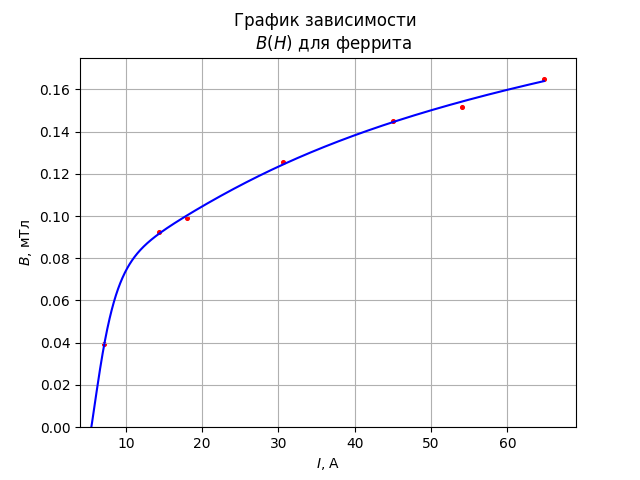
\includegraphics [scale=0.7]{3-4-5_Ferrit.png}}
		\caption{График зависимости $B(H)$ для феррита}
	\end{figure}
	
	\begin{figure}[h]
		\center{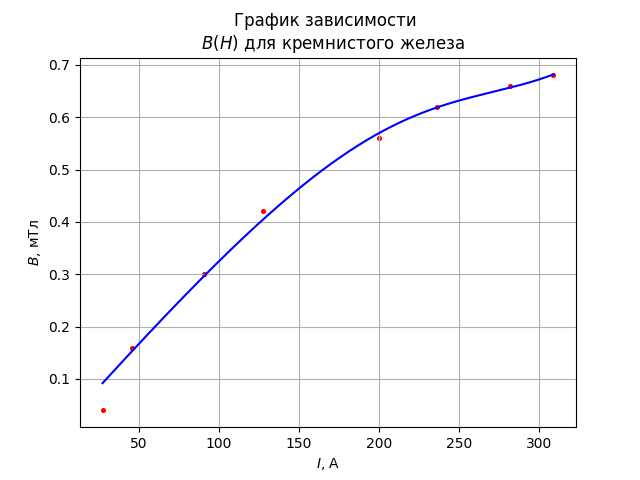
\includegraphics [scale=0.7]{3-4-5_KremnGeleso.png}}
		\caption{График зависимости $B(H)$ для кремнистого железа}
	\end{figure}
	
	\begin{figure}[h]
		\center{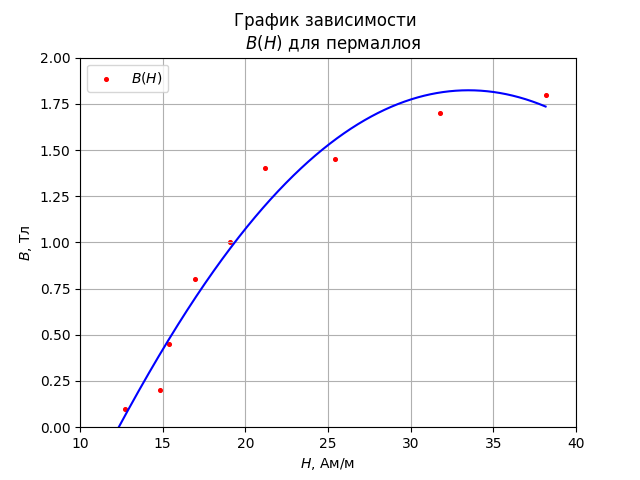
\includegraphics [scale=0.7]{3-4-5_Permalloiy.png}}
		\caption{График зависимости $B(H)$ для пермаллоя}
	\end{figure}



	
\end{document}